\documentclass[12pt]{article}
\usepackage{graphicx}
\usepackage{graphics}
\usepackage{refstyle}
\usepackage{amsmath}
\usepackage{caption}
\usepackage{float}
\usepackage{physics}
\usepackage{tasks}
\usepackage{listings}
\usepackage{gensymb}
\usepackage{textcomp, gensymb}
\usepackage{tabularray}
\usepackage[utf8]{inputenc}
\graphicspath{{/sdcard/Download/maths/figs}}
\newcommand{\myvec}[1]{\ensuremath{\begin{pmatrix}#1\end{pmatrix}}}
\let\vec\mathbf
%\renewcommand{\vec}[1]{\textbf{#1}}
\begin{document}
\begin{center}
 \section*{\textbf{Class 12}}
 \subsection*{Chapter 10 - Vector Algebra}
\end{center}
This is question 18 from exercise 10.5
\begin{enumerate}
\item  The value of  $\hat{i} \cdot (\hat{j} \times \hat{k})+\hat{j} \cdot (\hat{i} \times \hat{k})+\hat{k} \cdot (\hat{i} \times \hat{j})$ is
\begin{tasks}(4)
          \task $0$ 
          \task $-1$ 
          \task $1$ 
          \task $3$  
          \end{tasks}
\end{enumerate}
\textbf{Solution:}
The Directional vectors of $x,y$ and $z$ axes are given respectively 
\begin{align}
\vec{e_1} =\myvec{1\\0\\0}, \vec{e_2}=\myvec{0\\1\\0}, \vec{e_3} =\myvec{0\\0\\1}
\end{align}
Here,
$\vec{e_i} = \myvec{0\\0\\0\\1 (i^{\text{th}} term)\\0\\0\\0...}$, $\vec{e_j} = \myvec{0\\0\\0\\1 (j^{\text{th}} term)\\0\\0\\0...}$, $\vec{e_k} = \myvec{0\\0\\0\\1 (k^{\text{th}} term)\\0\\0\\0...}$ \\

\[
\begin{aligned}
\begin{tabular} {l|l}
$\vec{e_i} \times \vec{e_j} = \vec{e_k}$ &$\vec{e_j} \times \vec{e_i} = -\vec{e_k}$ \\
$\vec{e_j} \times \vec{e_k} = \vec{e_i}$ & $\vec{e_k} \times \vec{e_j} = -\vec{e_i}$ \\
$\vec{e_k} \times \vec{e_i} = \vec{e_j}$ &$\vec{e_i} \times \vec{e_k} = -\vec{e_j}$ \\
\end{tabular}
\end{aligned}
\] \\

\fbox{\begin{minipage}{15em}
$\vec{e_i}^{\top} \vec{e_i} = |\vec{e_i}| |\vec{e_i}| \cos{0} $ \\
                       = $ 1 \times 1 \times 1 $ \\
                       = $ 1 $ \\
similarly, $ \vec{e_j}^{\top} \vec{e_j} = \vec{e_k}^{\top} \vec{e_k} = 1$
\end{minipage}} \\
\\
Now,
\begin{center}  
$\vec{e_1}^{\top} (\vec{e_2} \times \vec{e_3})$ + $\vec{e_2}^{\top} (\vec{e_1} \times \vec{e_3})$ + $\vec{e_3}^{\top} (\vec{e_1} \times \vec{e_2} )$ \\
    = $ 1 - 1 + 1 $\\
    =$1$\\
\end{center}
So, option (c) is correct.

\begin{figure}[H]
        \centering
  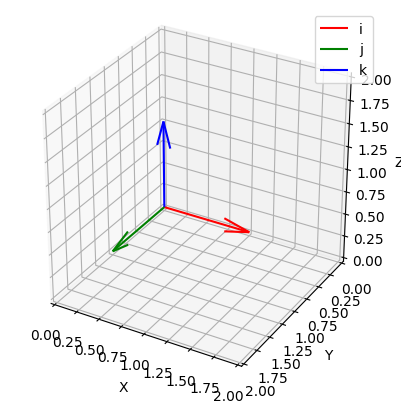
\includegraphics[width=\columnwidth]{figs/unit_vec.png}
                \label{fig:12/10/5/18}
         \caption{fig:1}
               \end{figure}
\end{document}
